\problemname{Tävlingssal}
När man anordnar en tävling för PO (Pragmatiska Ortogonalitetsföreningen) är
det viktigt att se till att deltagarna sitter strukturerat och samtidigt inte
sitter för nära varandra. På så sätt undviker man att
deltagarna blir störda av andra samtidigt som man motverkar fusk.
Arrangörerna har kommit fram till att deltagarna ska sitta i ett mönster som ser ut
som ett regelbundet rutnät med avståndet minst $1$ till närmaste granne (se bild nedan).
Avståndet från en deltagare ut till väggen ska också vara minst $1$.
Tävlingssalen ska dessutom vara en rektangel vars sidor är parallella med rutnätet.

Givet antalet deltagare $N$, bestäm minsta möjliga arean för tävlingssalen, givet att man placerar
deltagarna optimalt.

\section*{Input}
Ett heltal $N$ på en enda rad - antalet deltagare.

\section*{Output}
Skriv ut ett heltal på en enda rad - den minsta möjliga arean för tävlingssalen.

\section*{Förklaring av exempel}
Se Figure 1 för en förklaring av indataexemplet. De svarta pilarna illustrerar det nödvändiga avståndet
$1$ mellan deltagarna och väggarna.
\begin{figure}[ht!]
\centering
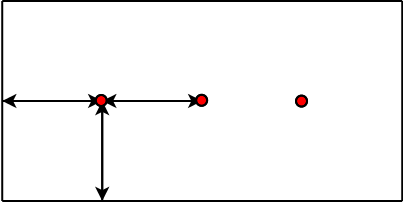
\includegraphics[width=0.4\textwidth]{tavlingssal.png}
\caption{En illustration av en optimal lösning för Sample Input 1.}
\label{overflow}
\end{figure}


\section*{Poängsättning}
Din lösning kommer att testas på en mängd testfallsgrupper. För att få poäng
för en grupp så måste du klara alla testfall i gruppen.

\begin{tabular}{| l | l | l | l |}
\hline
Grupp & Poängvärde & Gränser & Övrigt\\ \hline
1     & 40         & $ 1 \le N \le 1000 $ & \\ \hline
2     & 30         & $ 1 \le N \le 10^6 $ & \\ \hline
3     & 30         & $ 1 \le N \le 10^9 $ & \\ \hline
\end{tabular}
